% !TEX root = ../thesis_main.tex
%
%
%
%%%% --- * --- %%%%	
\clearpage
%\chapter{Calibrations and Analysis}
\chapter{Calibrations}

\note[color=org]{I have some tables summarizing which types of data were measured.  Presently, that's in Ch-4, but probably I should move it here.}



%%%% --- * --- %%%%	
%\section{Calibrations}
\label{calibrations_chapter}

\section{Measurements of the Atom Cloud}
\label{sec:cloud_calibration}

\note[color=org]{Content that previously was in this subsection is now in Section~\ref{cloud}.  But also, see Section~\ref{sec:photoprobe}.  Probably in this section here, I need to just jump right in assuming everyone understands the physical principle of how the data works.  Then, I can talk about what the data *is*, and how it gets interpreted.}

%\label{cloud}
%\label{photoions}
%\note[color=org]{Some of this stuff is in Ch.3 and/or Ch.4.  Some of it *should* be.}
%In order to measure properties of the trapped $^{37}\textrm{K}$ cloud, a 10\,kHz pulsed laser at 355\,nm is directed towards the cloud.  These photons have sufficient energy to photoionize neutral $^{37}\textrm{K}$ from its excited atomic state, which is populated by the trapping laser when the MOT is active, releasing 0.77\,eV of kinetic energy, but do not interact with ground state $^{37}\textrm{K}$ atoms.  The laser is of sufficiently low intensity that the great majority\aside[color=jb]{JB:  ``On order 1\% are photoionized."} of excited state atoms are \emph{not} photoionized, so the technique is only very minimally destructive.  
%\note{Probably worth mentioning that we test this stuff offline on stable \isotope[41]{K}. }
%
%
%Because an electric field has been applied within this region (see Section~\ref{field})\aside[color=jb]{JB:  ``you could reference the letter for the value of the field 150V/cm.''} the $^{37}\textrm{K}^+$ ions are immediately pulled into the detector on one side of the chamber, while the freed $e^-$ is pulled towards the detector on the opposite side of the chamber.  Because  $^{37}\textrm{K}^+$ is quite heavy relative to its initial energy, it can be treated as moving in a straight line directly to the detector, where its hit position on the microchannel plate is taken as a 2D projection of its position within the cloud.  Similarly, given a sufficient understanding of the electric field, the time difference between the laser pulse and the microchannel plate hit allows for a calculation of the ion's initial position along the third axis.  
%
%\note{As a check:  the camera measurements for photons from de-excitation.  It's aimed 35 degrees from vertical, with its horizontal axis the same as ..... one of the other axes.  I think it's the TOF axis.  I can check this when my computer comes back.   Also, there's an unknown additional delay between some of our DAQ channels that can't be explained by accounting for cable lengths, so we really like having the check there.}
%\note[color=jb]{JB says:  ``yes, camera x-axis is tof axis.''}
%
%
%With this procedure, it is possible to produce a precise map of the cloud's position and size, both of which are necessary for the precision measurements of angular correlation parameters that are of interest to us here.  However, it also allows us to extract a third measurement:  the cloud's polarization.
%
%The key to the polarization measurement is that only atoms in the excited atomic state can be photoionized via the 355 nm laser.  While the MOT runs, atoms are constantly being pushed around and excited by the trapping lasers, so this period of time provides a lot of information for characterizing the trap size and position.  When the MOT is shut off, the atoms quickly return to their ground states and are no longer photoionized until the optical pumping laser is turned on.  As described in Section~\ref{op}, and in greater detail in~\cite{ben_OP}, the optical pumping process involves repeatedly exciting atoms from their ground states until the atoms finally cannot absorb any further angular momentum and remain in their fully-polarized (ground) state until they are perturbed.  Therefore, there is a sharp spike in excited-state atoms (and therefore photoions) when the optical pumping begins, and none once\aside[color=jb]{JB points out that this should be ``if", not ``once".} the cloud has been completely polarized.  The number of photoion events that occur once the sample has been maximally polarized, in comparison with the size and shape of the initial spike of photoions, provides a very precise characterization of the cloud's final polarization~\cite{ben_OP}.



\note{Trap position -- Measured using the same dataset that was used to quantify the polarization.  The trap drifts slightly over the course of our data collection.  Describe the rMCP calibration needed to extract this info.}
\note{Polarization measurement was conducted on a different set of data, collected in between the measurements used for $A_{\mathrm{\beta}}$ and $b_{\mathrm{Fierz}}$, and at a higher electric field, because we were unable to run both our MCP detectors simultaneously.  }

\missingfigure{Need pictures of the cloud.  Possibly need projections of the cloud as a function of time, for AC/OP cycles.}
%\note{Need to describe how polarization works.  Needs a level diagram.  Needs another(?) level diagram for the photoionization, and maybe a third for the MOT.  Can I combine them all?  idk.}

Anyway, here is a nice table describing the atom cloud, for each of 3 runsets, and I'll immediately reference it right now, as Table~\ref{table:cloudpositions}:

% !TEX root = ../thesis_main.tex


\begin{table}[h!!!!t]
	\begin{center}
	\begin{tabular}{ c | r || lcl | lcl || lcl | lcl |}
	%	\hline
	%		\multicolumn{5}{ | c | }{Cloud Measurements -- $x$-Projection} \\
	%	\hline\hline
	%	\cline{3-6}
			\multicolumn{2}{  c  }{ } & 
				\multicolumn{3}{  c  }{ \!\!Initial Position\!\! } &  \multicolumn{3}{   c  }{ Final Position } &  \multicolumn{3}{   c  }{ Initial Size } &  \multicolumn{3}{   c  }{ Final Size } \\
		%	\cline{2-6}
		%	\hline
		%	\cline{2-6}
			\cline{2-14}
			\multirow{3}{*}{Runset B}  & $x$ & \,\,1.77 & \!\!$\!\! \pm  \!\!$\!\! & 0.03   & \,\,2.06   & \!\!$\!\! \pm  \!\!$\!\! & 0.08    & 0.601 & \!\!$\!\! \pm  \!\!$\!\! & 0.013 & 1.504 & \!\!$\!\! \pm  \!\!$\!\! & 0.047 \\
								& $y$ & -3.51    & \!\!$\!\! \pm  \!\!$\!\! & 0.04   & -3.33     & \!\!$\!\! \pm  \!\!$\!\! & 0.05    & 1.009 & \!\!$\!\! \pm  \!\!$\!\! & 0.013 & 1.551 & \!\!$\!\! \pm  \!\!$\!\! & 0.018 \\
								& $z$ & -0.661  & \!\!$\!\! \pm  \!\!$\!\! & 0.005 & -0.551   & \!\!$\!\! \pm  \!\!$\!\! & 0.021  & 0.891 & \!\!$\!\! \pm  \!\!$\!\! & 0.004 & 1.707 & \!\!$\!\! \pm  \!\!$\!\! & 0.015 \\
			\cline{2-14}
			\multirow{3}{*}{Runset C}  & $x$ & \,\,2.22  & \!\!$\!\! \pm  \!\!$\!\! & 0.05  & \,\,2.33   & \!\!$\!\! \pm  \!\!$\!\! & 0.11    & 1.18   & \!\!$\!\! \pm  \!\!$\!\! & 0.04   & 1.538 & \!\!$\!\! \pm  \!\!$\!\! & 0.087 \\
								& $y$ & -3.68     & \!\!$\!\! \pm  \!\!$\!\! & 0.04  & -3.31      & \!\!$\!\! \pm  \!\!$\!\! & 0.06   & 0.965 & \!\!$\!\! \pm  \!\!$\!\! & 0.012 & 1.460 & \!\!$\!\! \pm  \!\!$\!\! & 0.030 \\
								& $z$ & -0.437   & \!\!$\!\! \pm  \!\!$\!\! & 0.09  & -0.346    & \!\!$\!\! \pm  \!\!$\!\! & 0.037 & 0.927 & \!\!$\!\! \pm  \!\!$\!\! & 0.007 & 1.797 & \!\!$\!\! \pm  \!\!$\!\! & 0.026 \\
			\cline{2-14}
			\multirow{3}{*}{Runset D}  & $x$ & \,\,2.274 & \!\!$\!\! \pm  \!\!$\!\! & 0.012 & \,\,2.46 & \!\!$\!\! \pm  \!\!$\!\! & 0.06   & 0.386 & \!\!$\!\! \pm  \!\!$\!\! & 0.016 & 1.382 & \!\!$\!\! \pm  \!\!$\!\! & 0.046 \\
								& $y$ & -4.54      & \!\!$\!\! \pm  \!\!$\!\! & 0.04   & -4.28    & \!\!$\!\! \pm  \!\!$\!\! & 0.04   & 0.986 & \!\!$\!\! \pm  \!\!$\!\! & 0.08   & 1.502 & \!\!$\!\! \pm  \!\!$\!\! & 0.013 \\
								& $z$ & -0.587    & \!\!$\!\! \pm  \!\!$\!\! & 0.04   & -0.481  & \!\!$\!\! \pm  \!\!$\!\! & 0.018 & 0.969 & \!\!$\!\! \pm  \!\!$\!\! & 0.003 & 1.861 & \!\!$\!\! \pm  \!\!$\!\! & 0.013 \\
			\cline{2-14}
	\end{tabular}
	\end{center}
%	\label{table:cloudpositions}
	\note{These positions are for the *electron* runsets of those names.  Might want a chart of which rMCP runs are used to measure position for which eMCP runs.  Possibly in that other section.}
	\note{Sig figs here need work.}
	\caption[Cloud Position and Size]{Cloud Positions and Sizes -- Measured immediately before and immediately following the optical pumping phase of the trapping cycle.  All entries are expressed in units of mm, and the ``size" parameters describe the gaussian width.}
	\label{table:cloudpositions}
\end{table}




\note{Also, we noticed the trap drifting after one of the runs, because one of the batteries on one of the thingies adjusting the laser frequency (I think) was failing. }
\note[color=jb]{JB:  ``If we rejected the data with the MOT moving (indeed a battery determining the voltage controlled oscillator frequency offset between absorption in stable \isotope[41]{K} cell and the \isotope[37]{K} resonance) then that's all you need to say.''}
\note{describe how you'd turn this into a physical description of the cloud, with like a temperature and a sail velocity and shit.  with equations.}



\begin{figure}[h!!t]
	\centering
	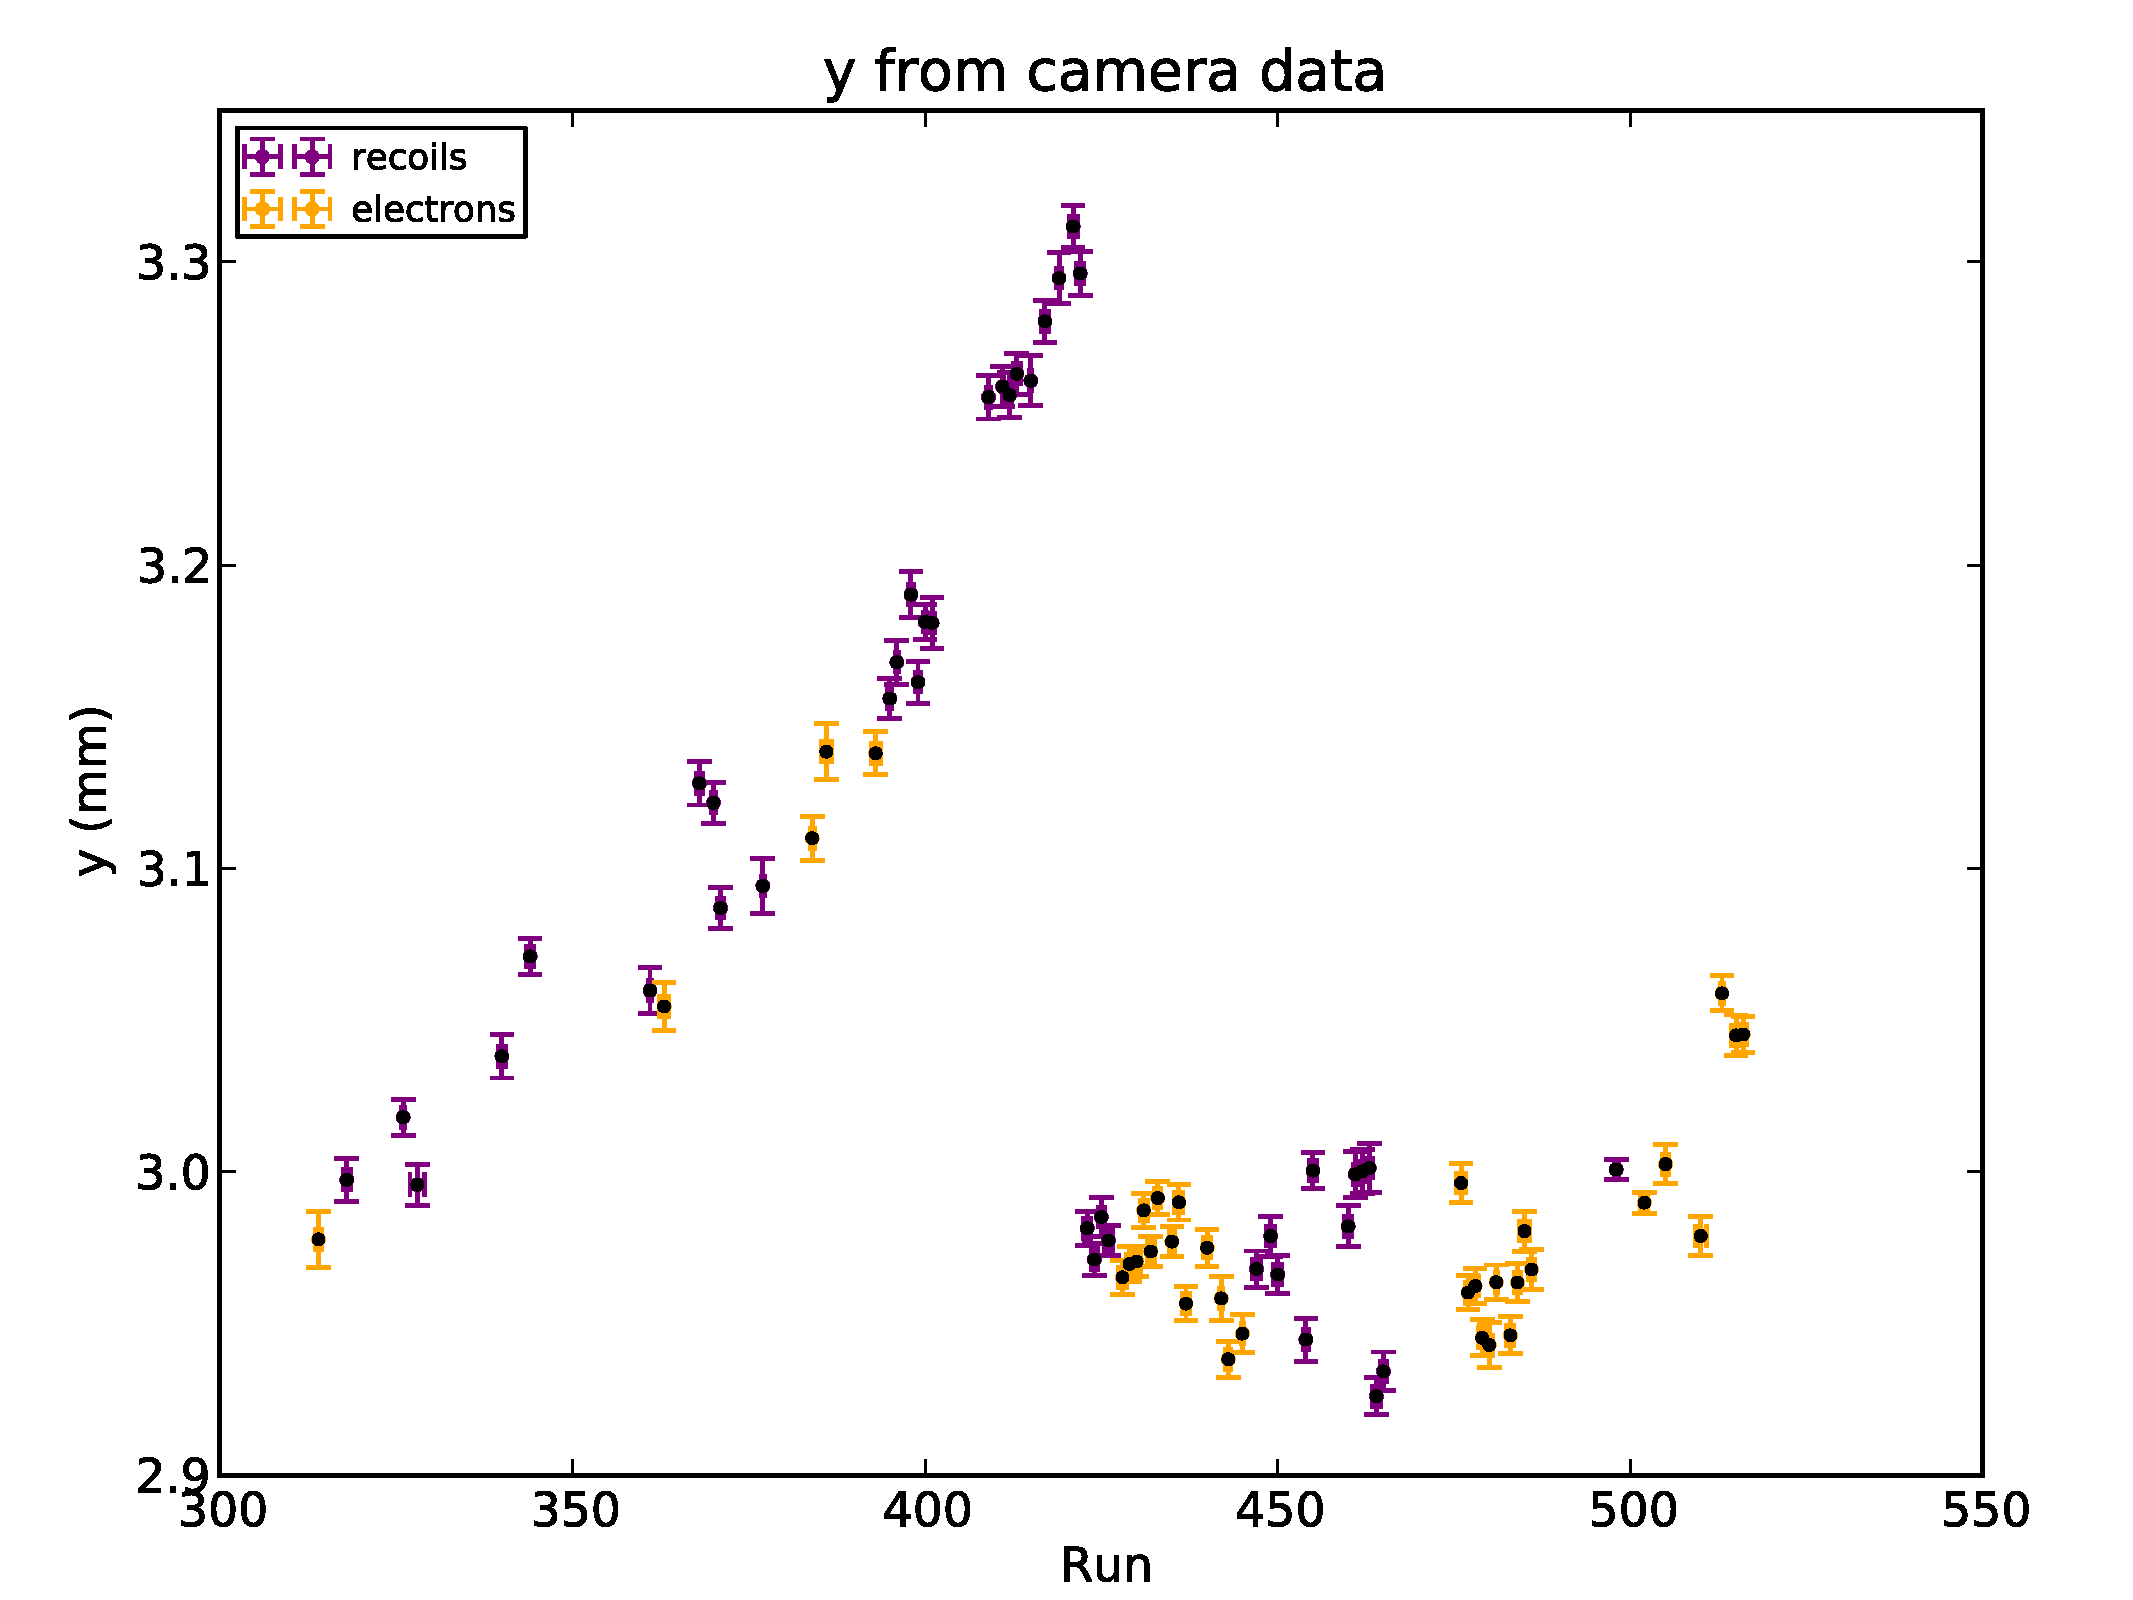
\includegraphics[width=.999\linewidth]
	{Figures/y_from_camera_electron_recoil.pdf}
	\caption[Trap Position along TOF Axis]{Trap Position along the ``Time-of-Flight'' Axis.  Electron runs and recoil runs plotted by run number. \comment{(I should probably re-plot this.  Maybe combine info with Fig.~(\ref{fig:cameraposition_by_time}).) } }	
	\label{fig:camera_electron_recoil}
\end{figure}

\begin{figure}[h!!t]
	\centering
	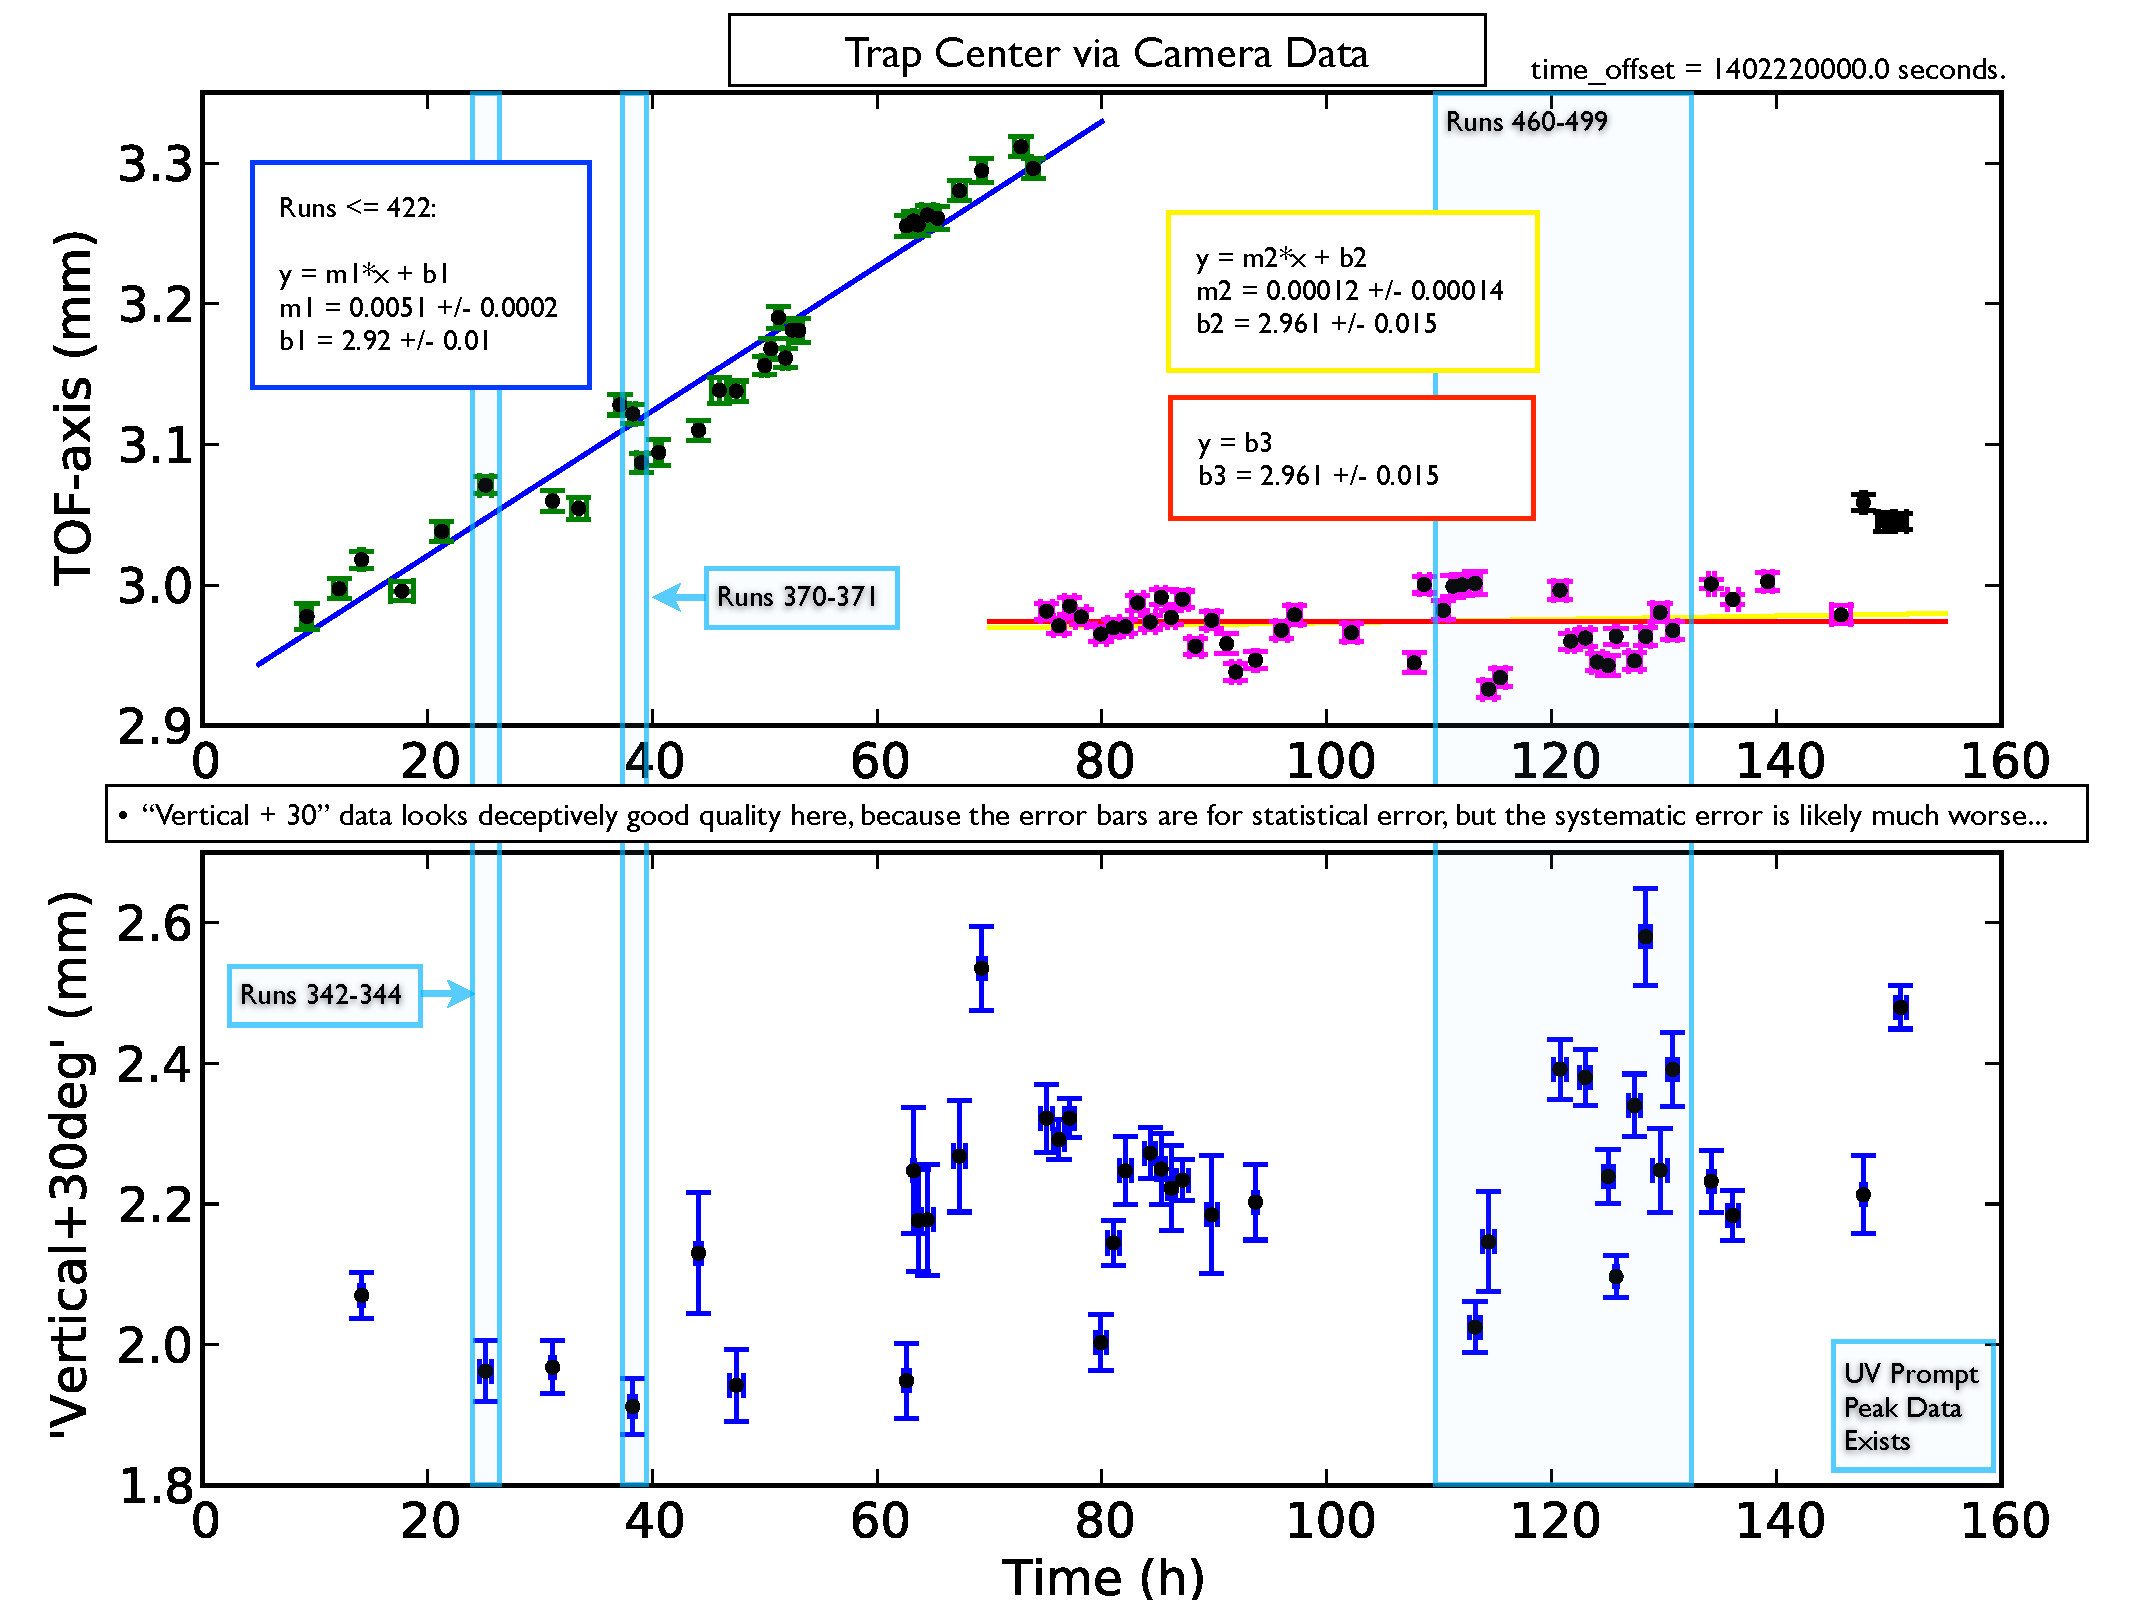
\includegraphics[width=.999\linewidth]
	{Figures/TrapPosition_FromCamera.pdf}
	\caption[Trap Position from Camera]{Trap Position along the ``Time-of-Flight'' Axis and the ``Vertical+30" Axis.  All runs plotted by time of run. \comment{(Need to re-plot this.)}}	
	\label{fig:cameraposition_by_time}
\end{figure}




\section{Beta Detector Cuts}
\label{section:calibrations_betadetectors}
	Setup is as described in Section~\ref{section:betadetectors}.	 
	\note{This is a stupid section name.  Also, I really do need to describe how the cuts were made here somewhere, because it's non-trivial in many cases, and possibly different than what Ben did in some cases.  But it won't make sense to describe what I did different if I don't describe the thing as a whole, at least a bit.  The point is, this is a set of cuts/systematics that isn't really that straightforward to understand.  }
%\section{Plastic Scintillators}
	\note[color=org]{Maybe this goes in Chapter~\ref{analysis_chapter}?}
	\note{Energy calibration for the scintillator+PMT setup changed dramatically at one point.    Describe how calibration was done.  Like, one sentence or something.  Something about the endpoint energy, and something about the compton edge for 511s, IIRC.}
	
%	Also describe how the DSSD calibration was done, even though it wasn't implemented by me. 
%	\note{How the fuck WERE these things done?!}
	\note[color=jb]{JB:  ``You can describe anything you did differently or improved, but you can and should otherwise defer all details of the scintillator calibration and DSSD calibration to Ben's paper and his thesis and Spencer's.  E.g. Section~\ref{section:bb1_systematics} ``statistical agreement between BB1 X and Y detectors' energies only makes a small effect on results" does not need the technical details beyond that statement."
	\label{thesisconventionjb} }
	\note[color=jb]{JB:  ``If you have some way of documenting the coding you used, that would be great."  ... yeah, it would, wouldn't it?}
%\section{Strip Detectors}
%	\note{How the fuck WERE these things done?!}



\section{The eMCP}
	I can describe the eMCP calibration here, even though it mostly wasn't implemented by me.  It is tangentially relevant to data selection and background estimation by providing an experimental energy spectrum for shake-off electrons.  It's actually a pretty neat algorithm that I basically wasn't involved with.
	\note[color=jb]{JB:  eMCP.  You need to describe the timing information obtained.  You also need a statement of whether or not you used the position information in your cuts.}

\missingfigure{Needs an SOE timing spectrum.  At least one of them.  Experimental and simulated.  Also, I have to describe how I did the simulating, and how I check that it's OK despite the fact that the simulated spectrum looks nothing like the experimental spectrum.}


\section{The rMCP}
	I did this, and they're absolutely needed to make any sense of the trap position data.  
%\missingfigure{Needs two pictures from the rMCP with the grid lines -- before and after corrections are performed.  Just for fun, I could throw in one with the stupid stripes.}
\begin{figure}[h!!t]
	\centering
	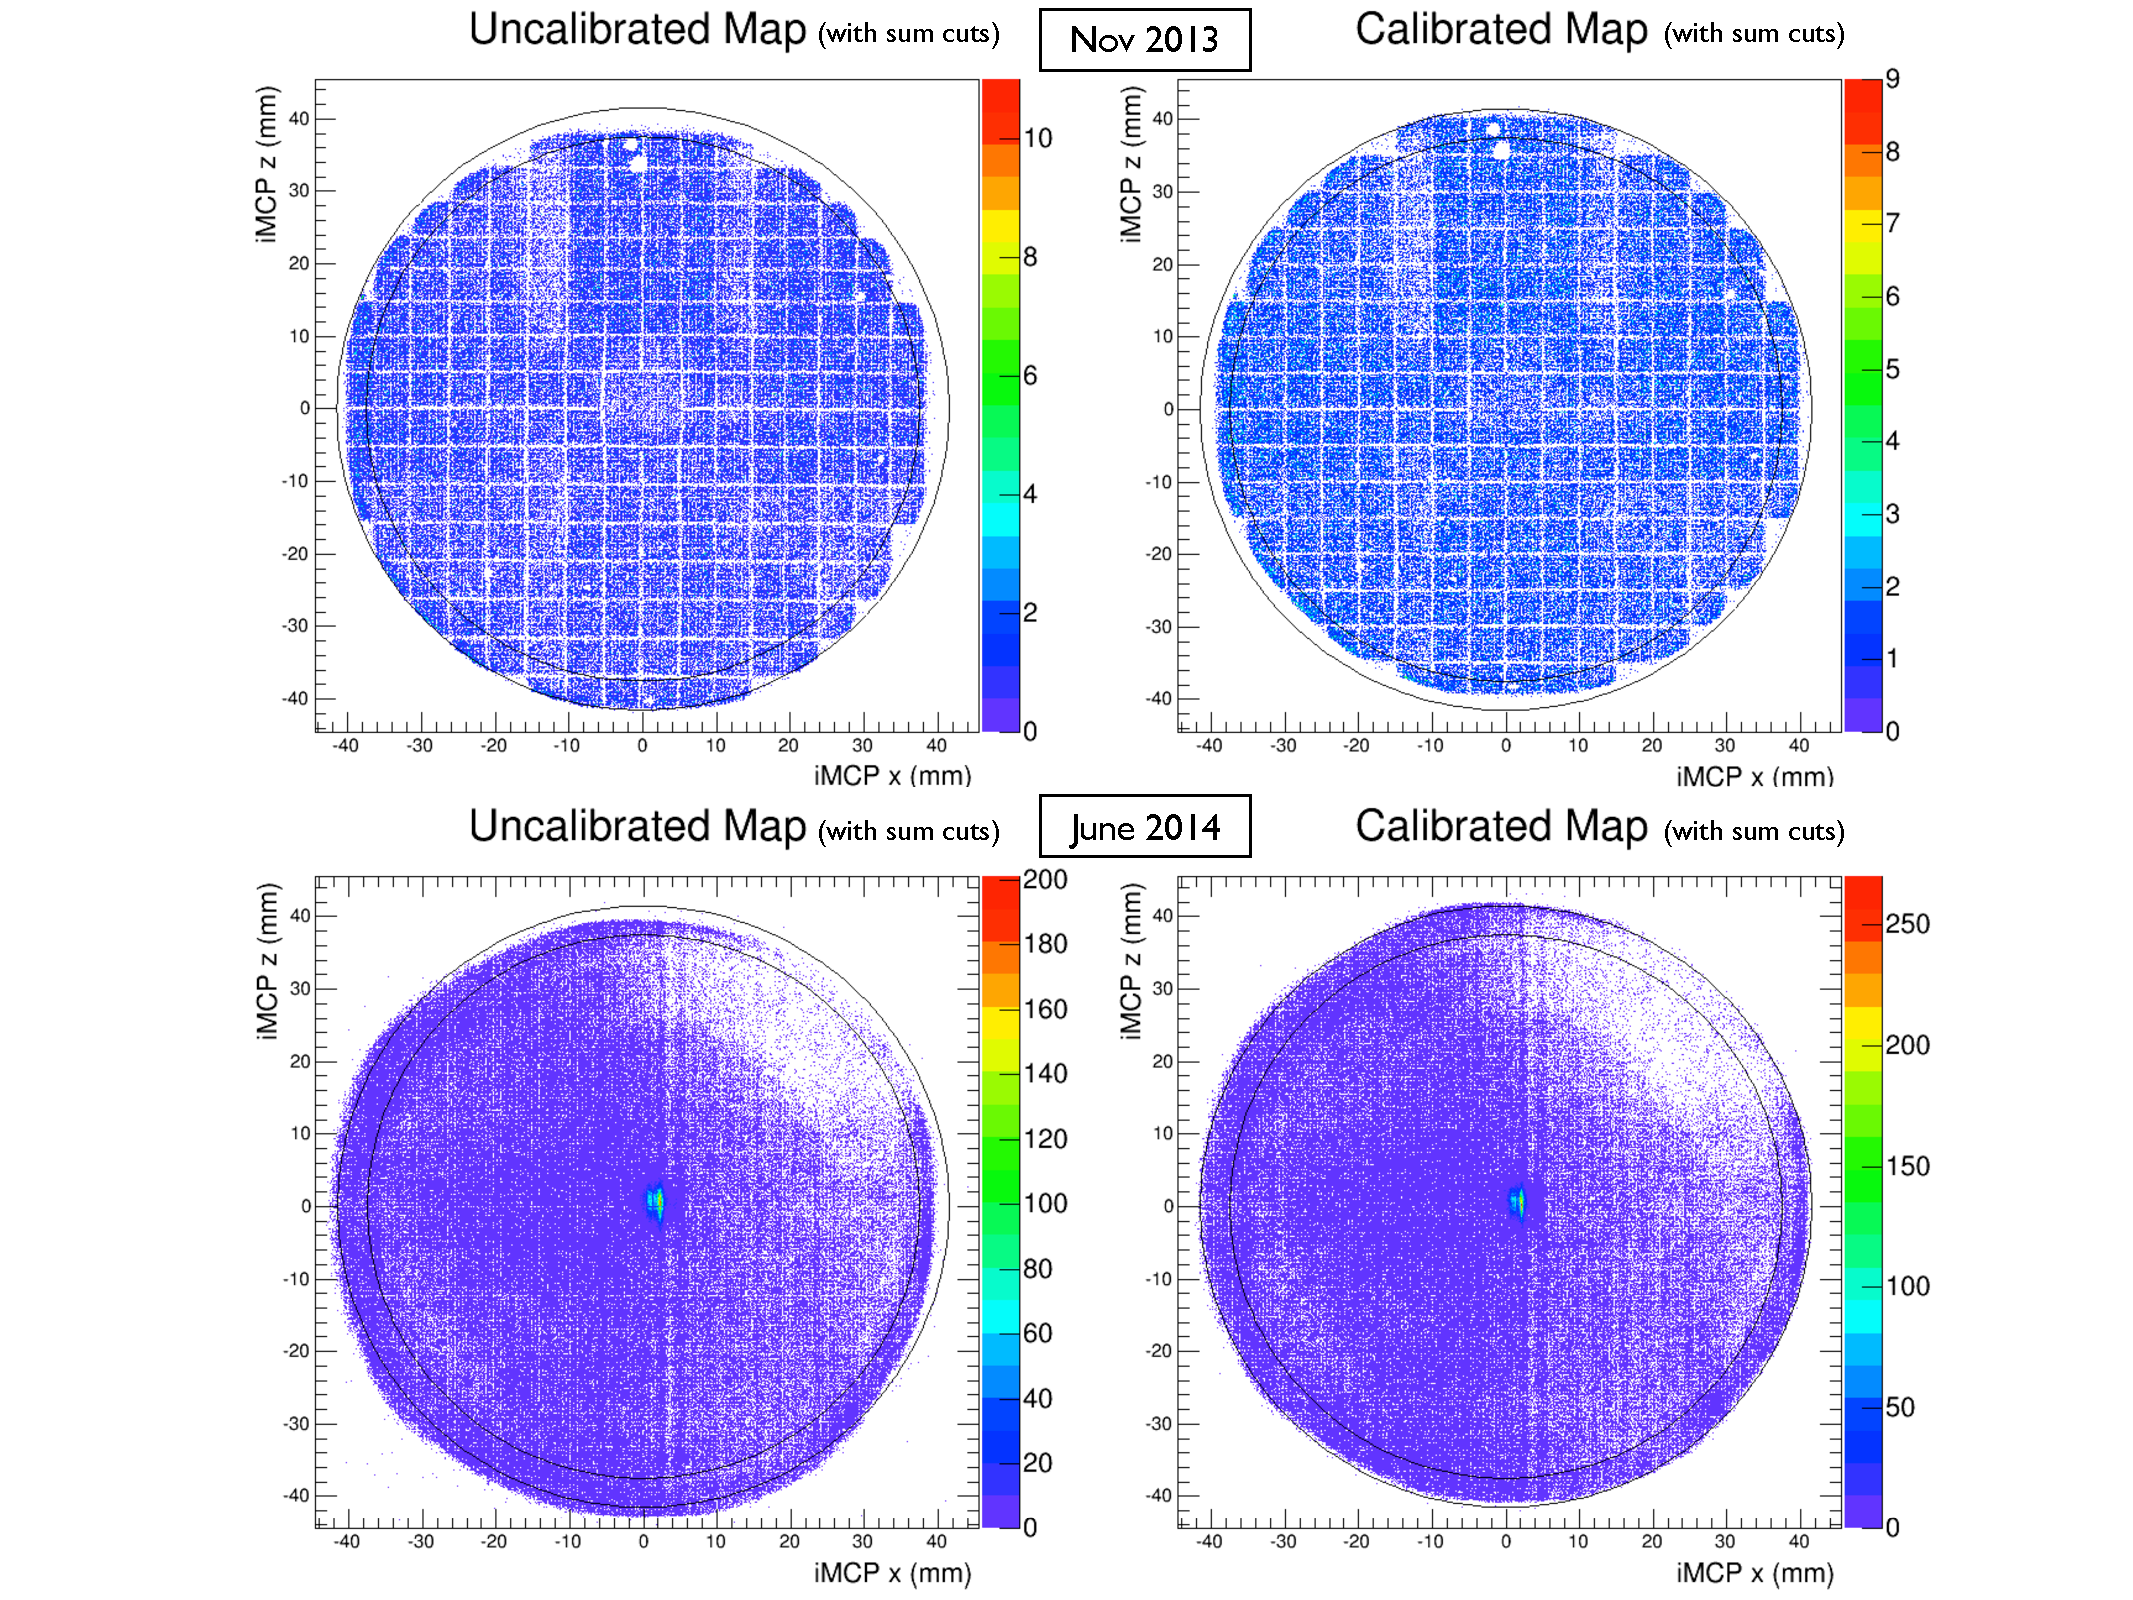
\includegraphics[width=.999\linewidth]
	{Figures/rMCP_Calibration}
	\caption[rMCP Calibration]{rMCP Calibration.  Definitely comment about how this calibration went here, in the figure caption. \comment{(Do I definitely want a picture with the stupid line-y runs?  Maybe it's better to just *not*...)}}	
	\label{fig:rmcp_calibration}
\end{figure}
	These calibrations are done during AC-MOT time, and we're actually interested in the rMCP data taken during OP time.  Can I find pictures to estimate the size of the change resulting from the magnetic field?  In any case, the change is pretty small.  

\subsection{rMCP Bullet Points!}
%	\begin{itemize}
%	\item 
	Using the ``other'' data set with the rMCP:  Measure the trap position/size/velocity/expansion with the rMCP and with the camera.  Necessitates calibrating the rMCP, which is its own whole thing.  Also measure polarization.
		\begin{itemize}
		\item rMCP calibration probably gets its own section, if not its own chapter..
		\item We took the mask off before the 2014 run, to give us more detector area.  Use previous reference calibration \emph{with the mask} during the test run in Nov 2013.  The delay line's non-linearities should be the same, assuming we can get the centering the same.  Cables have changed and stuff, so we have to re-center the pre-calibration image to where the old pre-calibration image was.  ...  So, center the new runs w.r.t the old run.
		\item We'll want to make some sum cuts for these things.  We might like them to be identical, or at least identical-ish, but the peaks don't really look the same.  So we'll settle for ``decent sum cuts for all!".  ...  So, apply sum cuts to the new runs and old run.
		\item Calibrate the old run, with the mask.  In fact, I don't remember which order I did things in.  But I have a record of it here, somewhere...
		\end{itemize}
%	\end{itemize}

%\missingfigure{Position as a function of run number.  I have this somewhere.}


%%%% --- * --- %%%%	
\clearpage
\chapter{Analysis}
\label{analysis_chapter}

\section{Data Selection and Pre-Processing}
Although the detection chamber was designed to feature two MCP detectors on opposing sides of an applied electric field intended for simultaneous use (see Section~\ref{section:mcps}), % to collect positively charged recoiling ions on the rMCP and negatively charged shake-off electrons on the eMCP 
in practice the two detectors produced quite a bit of feedback when operated at the same time.  In order to salvage usable data from the beamtime, we ended up running only one detector at a time, but switched which detector was in use every few hours, collecting approximately the same amount of data with each detector.  Thus, the runs are sorted into `electron' and `recoil' runs, depending on what the detector in use was intended to detect.  

While the beta asymmetry and Fierz interference are best evaluated using the electron runs, the recoil runs are best for evaluating the polarization (a dominant uncertainty in the beta asymmetry measurement) and the cloud position.  The polarization measurement is the subject of a recent publication (see~\cite{ben_OP}), and the cloud position evaluation is discussed in more detail in Chapter~\ref{calibrations_chapter}.

The data is further split up into four runsets:  A, B, C, and D based on when certain detection settings were adjusted, and each of these runsets contains both electron and recoil runs.  These four runsets were then treated separately for nearly all parts of the analysis.  In particular, Data Set A was neglected completely during analysis after it was determined that one scintillator had an improperly set hardware threshold such that lower energy betas weren't being detected at all.  Additionally, there was a QDC module failure between Runsets B and C, resulting in an abrupt change in calibration for the two scintillators.  
\note{Also, the background was too noisy in Set A I think.  Also, pretty sure there isn't really that much data in Set A at all.  Also-also, Set A has E=66.7, so can't use it for more stats on the other backgrounds. } 

%\note{What did I change between Runsets B and C?  Between Runsets C and D?  ...OP time, yes, but also and one point a PMT(?) (eta:  it was a QDC) blew out and we replaced it, so then the scintillator calibration was a bit different afterward.  Anyway, I should maybe just make a goddamn table.  Table goes here.}

% !TEX root = ../thesis_main.tex


\begin{table}[h!!!!t]
	\begin{center}
	\begin{tabular}{ c || p{5cm} | p{5cm} | p{1.2cm} | }
			\multicolumn{1}{  c  }{ } & 
				\multicolumn{1}{  c  }{ \!\!Electron Runs\!\! } &  \multicolumn{1}{   c  }{ Recoil Runs }  &  \multicolumn{1}{   c  }{ OP Delay }  \\
			\cline{2-4}
			\multirow{1}{*}{Runset A}	& 314, 362, 363, 383, 384, 385, 386, 393, 420.
									%	& 303, 308, 309, 310, 311, 312, 313, 318, 326, 327, 328, 340, 342, 343, 361, 368, 370, 371, 376, 377, 378, 394, 395, 396, 398, 399, 400, 401, 402, 409, 410, 411, 412, 413, 414, 415, 416, 417, 418, 419.
										& 303, 308-313, 318, 326, 327, 328, 340, 342, 343, %361, 368, 370, 371, 
										376, 377, 378, 394, 395, 396, 398-402, 409-419.
										& $300\,\mu s$
										\\
			\cline{2-4}
			\multirow{1}{*}{Runset B}	& 428-437, 440-445.
										& 421-426, 446, 447, 449.
										& $300\,\mu s$
										\\
			\cline{2-4}
			\multirow{1}{*}{Runset C}	& 476, 477.
										& 450, 454, 455, 460-466, 473, 474.
										& $700\,\mu s$
										\\
			\cline{2-4}
			\multirow{1}{*}{Runset D}	& 478-489, 502, 503, 504, 505, 510, 513.
										& 491, 497, 498, 499, 509.   
										& $400\,\mu s$
										\\
			\cline{2-4}
	\end{tabular}
	\end{center}
	\note{MUST check to make sure I didn't use Run 420 in ``good runs" in the end!!!}
	\note{I have more (really early) runs classed in Set A than Ben had.  In the end, we didn't use them so it doesn't matter.  But...what?}
	\note{Ugh.  My categorization system is slightly different than Ben's on the later recoils.  That's annoying.}
	\note{Other things I could list here:  Electric field strengths, total runtime.}
	\caption[List of Runs]{A list of 2014 online runs with potentially usable data.  Runset A was discarded completely due to problems with hardware threshold settings.  There was a QDC module failure before Run 450, so it and all subsequent runs were performed using a different module, and as a result the scintillator calibrations changed slightly at this time.  Anyway, the point of this thing is to show which electron runs and recoil runs go together, for the purposes of evaluating polarization and cloud attributes.}
	\label{table:runlist}
\end{table}



Before proceeding further, several basic cuts are performed on the data.  For the Electron Runs which are to be processed directly into a physical measurement, we consider only events in which there was a recorded hit \emph{both} on the eMCP \emph{and} on (at least) one of the scintillators.  The required scintillator hit, of course, is potentially a beta, and so it is obvious why this must be present.  The eMCP hit requirement -- particularly with the timing of the eMCP hit occuring within a certain time range relative to the scintillator hit -- is used to tag beta decay events originating from the cloud, as opposed to those originating from some other surface within the chamber.  The precise time interval to be used, and how its results should be evaluated,\aside{also discussed: how we decide what counts as an eMCP hit at all} is discussed in Section~\ref{something}, but for the first pass through the data it is good enough to simply require that an eMCP hit occurred.\aside{Awkward stupid phrasing.}  Although not every beta decay event from the cloud will produce a hit on the eMCP, this requirement eliminates a great deal of background that would otherwise be challenging to evaluate.  \aside{Also, we claim that it doesn't bias the data.  Much.  Didn't I try to evaluate how much it biased the data at one point?}  
 
%The scintillator hit is considered to be potentially a beta from a decay
Because the eMCP hit is required as a `tag' of good events, it is also necessary to remove from direct consideration any event which is coincident with a pulse of the photoionization laser.  When photoionization occurs within the atom cloud, an orbital electron is removed from the atom and will be accelerated by the electric field into the eMCP, just as a shake-off electron from a decay might be.  If, by chance, this photoelectron arrives in coincidence with a scintillator hit, it would be interpreted as a decay event from the trap -- unless we preemtively discard it.  


Over the course of the runtime, there were several instances where we noted an apparent electrical discharge within the experimental chamber, producing enormous backgrounds for a short time.  The detectors typically recovered quickly afterward, so it was neither necessary nor useful to stop an entire run to wait for the system to recover.  Instead, the time when the discharge occurred was recorded, and events within approximately one minute of the spark time were discarded.  

%Because it is of the utmost importance to understand the nuclear spin-polarization immediately prior to a decay, 
We use only the ``fully polarized'' events for which we have a detailed understanding of the nuclear polarization (described in more detail in ~\cite{ben_OP}).  This means we must use \emph{only} events from the ``optical pumping'' portion of the duty cycle (see Fig.~\ref{fig:dutycycle}), and discard events when the DC- or AC-MOT is active.  After the AC-MOT is shut off, there is a short delay before optical pumping begins (see Table~\ref{table:runlist}) to allow the magnetic field to decay, and it is only after $100\,\mu s$ of optical pumping that we consider the atoms to be fully polarized.  Furthermore, because the magnetic field from the DC-MOT is slow to decay (relative to the field from the AC-MOT), all events from the first five AC/OP cycles after every atom transfer are discarded.  A secondary benefit of our insistence on considering only polarized data is that the scintillators' gains are more stable in the presence of only the (small, stable) magnetic field used for optical pumping than they are in the presence of a larger oscillating magnetic field used for trapping.
\note{change by 0.2\% of its value vs change by 0.5\% of its value, according to Ben's thesis pg 143.}

%Another class of event that must be removed from direct analysis is 
Finally, because this analysis depends heavily on energy measurements from the two scintillators as a proxy for beta energy, it is necessary to remove events in which the pulser LED fired.  Although the pulser LED is useful for evaluating the stability of the scintillators, in the case where an LED pulse occurs together with a true beta hit in the scintillator, it may change the measured energy.  Therefore, we discard all events that include an LED pulse.   
	

\section{Further Cuts Using the DSSD}



\section{Further Cuts Using the eMCP}



\section{Bullet Points!}
Right, so.  Here's how I processed the data into an answer.  In bullet point form, so I don't forget stuff while I'm obsessively trying to phrase everything well.  
\newline

With the Data:
\begin{itemize}
	\item \greycomment{Lower-level data cleaning.  Discard events during parts of the duty cycle when atoms weren't polarized.  Discard events near a recorded spark time. Discard events when the photoionization laser fires.  Discard events when the LED pulser used to calibrate the scintillators fires.}
	\item \greycomment{Split up runs into sets, to account for changing experimental conditions.  Possibly I should list what the differences between runs were somewhere.  But not in this section.  OTOH, ...maybe?}
	%
	\item Make some more careful cuts to clean the data.  
		\begin{itemize}
		\item Discard events without a ``good'' DSSD hit.  Eliminates vast majority of background 511s.  Necessitates having a definition of what a ``good'' DSSD hit is.  It's subtle enough that we'll want to leave some part of this definition of ``good'' to be varied as a systematic effect.  Notably, we consider energy agreement for each hit pixel, individual strip SNR, and overall DSSD energy threshold.  Also, hit radius w.r.t. center of detector.  This is a lot of stuff, all implemented by Ben -- and it needs to be done fairly early on in data processing in order to keep processing times for everything else manageable.  
		\item Discard events where SOE-Beta TOF falls outside a certain range.  Necessitates picking a ``good'' range.  The precise definition of ``good'' is varied as a systematic.
		\end{itemize}
\end{itemize}

\vspace{24pt}
\vspace{12pt}
With the Simulations:
\begin{itemize}
	\item Update G4 event generator to be able to model non-zero scalar and tensor coupling.  These things show up in $\Abeta$ too, not just in $\bFierz$.  Though, the effects on $\Abeta$ are much smaller.
	\item Run 3 sets of G4 simulations with a bunch of statistics (N events, for data with like N/10 events).  Each one has the same nominal value of $\Abeta$, but with 3 different values of the scalar coupling $C_S$:  zero, and +/-(whatever).  Keep $C_T=0$.  Because reasons, we're not really able to distinguish between $C_S$ and $C_T$ in this experiment anyway, so might as well keep the analysis simple.
	\item Just run one set of 0.02*N events for the two percent branch.  We can't neglect it, but it isn't going to change (much?) when we adjust BSM couplings.
	\item Match cuts in simulated data up to the cuts on experimental data.  Obviously.  DSSD cut, DSSD energy, one hit DSSD, one hit scint.  TOF cut, which requires a whole extra model of background in the TOF spectrum..
		\begin{itemize}
		\item Suppose background in the TOF spectrum is coming from decays of atoms that have gotten themselves stuck to surfaces within the chamber...
		\item Run G4 to get a beta TOF spectrum (w.r.t. the decay)
		\item Run COMSOL (credit to Alexandre) to track low-energy SOEs through the electric field from wherever they started, into the detectors.  Energy spectra from Levinger.
		\item Combine G4 and COMSOL spectra, event-by-event, while requiring that both the beta detector and the eMCP are hit according to the set of random numbers generated by each monte carlo separately.  Then, the beta and SOE will each have a TOF from decay to detector, and subtracting one from the other gives a timing spectrum that can be observed experimentally.  See Fig.~\ref{fig:soetof}.
		\item Upper limit for the fraction of events generated this way can be estimated by assuming that all losses from the trap not due to radioactive decay emerge isotropically from the trap and then stick to whatever chamber wall is in its path.  This upper limit is too big by a factor of 2.
		\end{itemize}
	\item For each of those 3 simulations, sort the ``good'' data according to emission angle relative to the detector.  Do each detector individually.  For both polarizations.
	\item Assemble the (simulated) superratio asymmetry.  We'll compare it to data, and the $\chi^2$ from that comparison will be our figure of merit.  
	\item We can make a whole 2D parameter space for different values of $\Abeta$ and $\bFierz$, and compare them all (via their superratio asymmetries) to the experimental data.  We get the ``best'' values of $\Abeta$ and $\bFierz$, where $\chi^2$ is minimized.
	\item We can do this whole thing again for simulated data sets with different values of parameters that we vary as systematics.  Note how the best values of $\Abeta$ and $\bFierz$ change when each of the systematics are varied.
	\item Then there's the lineshape thing.  My god, this wasn't nearly as useful as I thought it was going to be.  Certainly not worth the whole goddamn year that I spent on it.
\end{itemize}


\begin{figure}[t!h]
	\centering
	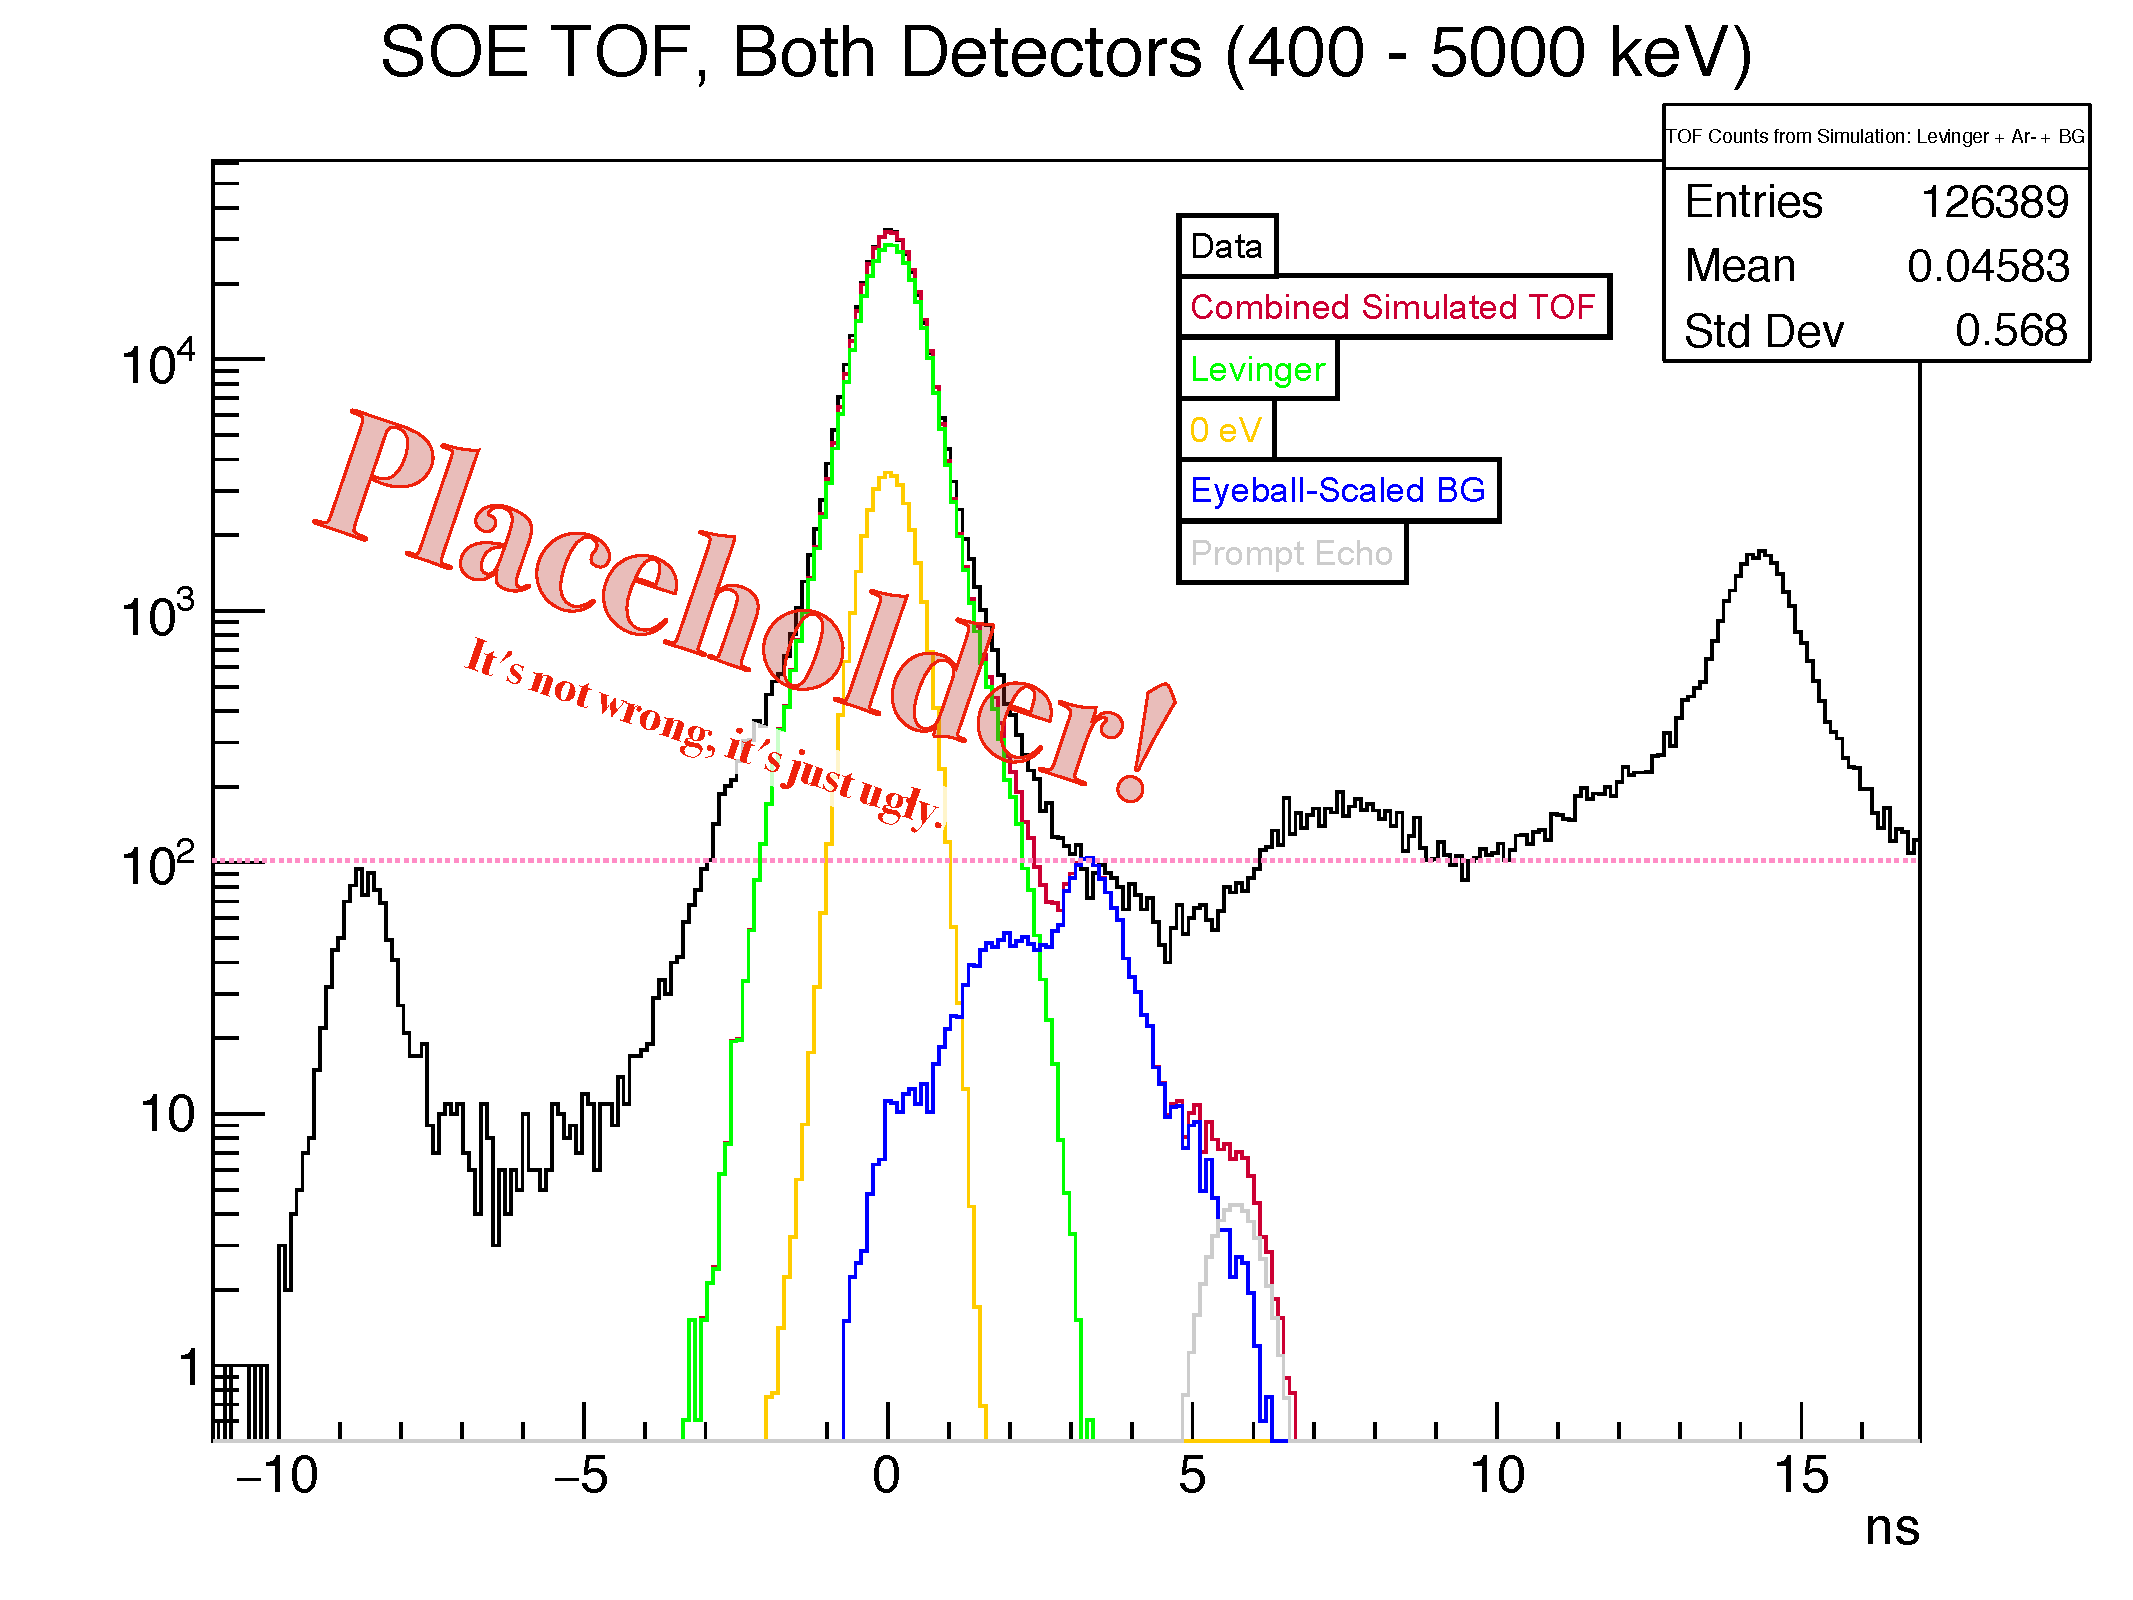
\includegraphics[width=.999\linewidth]
	{Figures/SOETOF_withmodel.pdf}
	\caption{SOE TOF, model and data.  In the end, I cut the data to use only events with a TOF between \comment{A and B.\;\;}  Max. possible background is like a factor of two too big.}	
	\label{fig:soetof}
\end{figure}



